\let\negmedspace\undefined
\let\negthickspace\undefined
\documentclass[journal]{IEEEtran}
\usepackage[a5paper, margin=10mm, onecolumn]{geometry}
\usepackage{tfrupee} 

\setlength{\headheight}{1cm} 
\setlength{\headsep}{0mm}  
\usepackage{gvv-book}
\usepackage{gvv}
\usepackage{cite}
\usepackage{amsmath,amssymb,amsfonts,amsthm}
\usepackage{algorithmic}
\usepackage{graphicx}
\usepackage{textcomp}
\usepackage{xcolor}
\usepackage{txfonts}
\usepackage{listings}
\usepackage{enumitem}
\usepackage{mathtools}
\usepackage{gensymb}
\usepackage{comment}
\usepackage[breaklinks=true]{hyperref}
\usepackage{tkz-euclide} 
\usepackage{listings}
% \usepackage{gvv}                                        
\def\inputGnumericTable{}                                 
\usepackage[latin1]{inputenc}                                
\usepackage{color}                                            
\usepackage{array}                                            
\usepackage{longtable}                                       
\usepackage{calc}                                             
\usepackage{multirow}                                         
\usepackage{hhline}                                           
\usepackage{ifthen}                                           
\usepackage{lscape}
\usepackage{tikz}
\usetikzlibrary{patterns}
\begin{document}

\bibliographystyle{IEEEtran}
\vspace{3cm}


\title{GATE 2009 ME }
\author{ee25btech11029- Jnanesh Sathisha Karmar}
\maketitle
% \maketitle
% \newpage
% \bigskip
{\let\newpage\relax\maketitle}

\renewcommand{\thefigure}{\theenumi}
\renewcommand{\thetable}{\theenumi}
\setlength{\intextsep}{10pt} % Space between text and floats
\begin{enumerate}[leftmargin=0pt]
    


        

% Q1
\item For a matrix $\sbrak{M}=\myvec{ \frac{4}{5} & \frac{3}{5} \\ \frac{3}{5} & x }$, the transpose of the matrix is equal to the inverse of the matrix, i.e., $\sbrak{M}^T=\sbrak{M}^{-1}$. The value of $x$ is given by:
  \begin{enumerate}
    \begin{multicols}{5}
        \item $4$
        \item $5$
        \item $-\frac{3}{5}$
        \item $\frac{3}{5}$
        \item $\frac{4}{5}$
    \end{multicols}
  \end{enumerate}
  \hfill{\brak{\text{GATE ME 2009}}}


% Q2
\item The divergence of the vector field $3 x z \hat{i} + 2 x y \hat{j} - y z^{2} \hat{k}$ at a point $\brak{1,1,1}$ is equal to:
  \begin{enumerate}
    \begin{multicols}{4}
        \item $7$
        \item $4$
        \item $3$
        \item $0$
        
    \end{multicols}
        
  \end{enumerate}
  \hfill{\brak{\text{GATE ME 2009}}}

% Q3
\item The inverse Laplace transform of $\frac{1}{s^{2} + s}$ is:
  \begin{enumerate}
    \begin{multicols}{4}
        \item $1 + e^{t}$
        \item $1 - e^{t}$
        \item $1 - e$
        \item $1 + e$
    \end{multicols}
  \end{enumerate}
  \hfill{\brak{\text{GATE ME 2009}}}

% Q4
\item If three coins are tossed simultaneously, the probability of getting at least one head is:
  \begin{enumerate}
    \begin{multicols}{4}
    \item $\frac{1}{8}$
    \item $\frac{3}{8}$
    \item $\frac{1}{2}$
    \item $\frac{7}{8}$
    \end{multicols}
  \end{enumerate}
  \hfill{\brak{\text{GATE ME 2009}}}


% Q5
\item If a closed system is undergoing an irreversible process, the entropy of the system:
  \begin{enumerate}
    \item must increase
    \item always remains constant
    \item must decrease
    \item can increase, decrease or remain constant
  \end{enumerate}
  \hfill{\brak{\text{GATE ME 2009}}}

% Q6
\item A coolant fluid at $30^\degree$C flows over a heated flat plate maintained at a constant temperature of $100^\degree$C. The boundary layer temperature distribution at a given location may be approximated as $T = 30 + 70 e^{-y}$ where $y$ \brak{\text{in} m} is the distance normal to the plate and $T$ is in $^\degree$C. If thermal conductivity is $1.0\,\mathrm{W/mK}$, the local convective heat transfer coefficient $\brak{\text{in} W/m^2K}$ at that location will be:
  \begin{enumerate}
    \begin{multicols}{4}
    \item $0.2$
    \item $1$
    \item $5$
    \item $10$
    \end{multicols}
  \end{enumerate}
  \hfill{\brak{\text{GATE ME 2009}}}

% Q7
\item A frictionless piston-cylinder device contains a gas initially at $0.8$ MPa and $0.015$ m$^3$. It expands quasi-statically at constant temperature to a final volume of $0.030$ m$^3$. The work output \brak{\text{in} kJ} during this process will be:
  \begin{enumerate}
    \begin{multicols}{4}
    \item $8.32$
    \item $12.00$
    \item $554.67$
    \item $8320.00$
    \end{multicols}
  \end{enumerate}
  \hfill{\brak{\text{GATE ME 2009}}}

% Q8
\item In an ideal vapor compression refrigeration cycle, the specific enthalpy of refrigerant $\brak{\text{in} kJ/kg}$ at the following states is given as: \\inlet of condenser: 283 \\exit of condenser: 116\\ exit of evaporator: 232.\\ The COP of this cycle is:
  \begin{enumerate}
    \begin{multicols}{4}
    \item $2.27$
    \item $2.75$
    \item $3.27$
    \item $3.75$
    \end{multicols}
  \end{enumerate}
  \hfill{\brak{\text{GATE ME 2009}}}

% Q9
\item A compressor undergoes a reversible, steady flow process. The specific work required to be supplied to the compressor for this gas compression process is:
  \begin{enumerate}
    \begin{multicols}{4}
    \item $\displaystyle \int_{1}^{2} P \, dv$
    \item $\displaystyle \int_{1}^{2} v \, dP$
    \item $v_1 \brak{P_2-P_1}$
    \item $-P_1\brak{v_1 - v_2}$
    \end{multicols}
  \end{enumerate}
  \hfill{\brak{\text{GATE ME 2009}}}


% Q10
\item A block weighing 981 N is resting on a horizontal surface. The coefficient of friction is $\mu=0.2$. A vertical cable provides partial support. A man can pull horizontally with 100 N. What will be the tension $T$ \brak{\text{in} N} in the cable if the man is just able to move the block to the right?

    \begin{figure}[h]
      \centering
      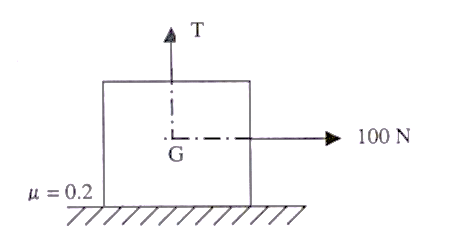
\includegraphics[width=0.5\textwidth]{Figs/image (2).png}
      \caption{}
      \label{fig:10}
    \end{figure}



  \begin{enumerate}
    \begin{multicols}{4}
    \item $176.2$
    \item $196.0$
    \item $481.0$
    \item $981.0$
    \end{multicols}
  \end{enumerate}
  \hfill{\brak{\text{GATE ME 2009}}}

% Q11
\item If the principal stresses in a plane stress problem are $\sigma_1 = 100$ MPa, $\sigma_2 = 40$ MPa, the magnitude of the maximum shear stress $\brak{in MPa}$ will be:
  \begin{enumerate}
    \begin{multicols}{4}
    \item $60$
    \item $50$
    \item $30$
    \item $20$
    \end{multicols}
  \end{enumerate}
  \hfill{\brak{\text{GATE ME 2009}}}

% Q12
\item A simple quick return mechanism is shown. If the forward to return ratio is 2:1, and radius of the crank $\vec{O_1P}$ is 125 mm, the distance $d$ \brak{\text{in} mm} between crank center to lever pivot center point should be
    \begin{figure}[h]
      \centering
      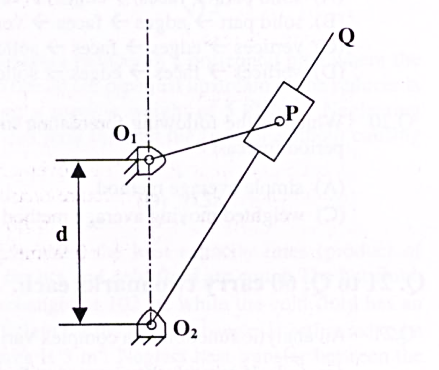
\includegraphics[width=0.3\linewidth]{Figs/image (3).png}
      \caption{}
      \label{fig:12}
    \end{figure}
    
  \begin{enumerate}
    \begin{multicols}{4}
    \item $144.3$
    \item $216.5$
    \item $240.0$
    \item $250.0$
    \end{multicols}
  \end{enumerate}
  \hfill{\brak{\text{GATE ME 2009}}}


% Q13
\item The rotor shaft of a large electric motor supported between short bearings at both ends shows a deflection of 1.8 mm. The likely critical speed $\brak{\text{in} \  rpm}$ is:
  \begin{enumerate}
    \begin{multicols}{4}
    \item $350$
    \item $705$
    \item $2810$
    \item $430$
    \end{multicols}
  \end{enumerate}
  \hfill{\brak{\text{GATE ME 2009}}}

% Q14
\item A solid circular shaft of diameter $d$ is subjected to a combined bending moment $M$ and torque $T$. The material property to be used for designing the shaft using the relation $\dfrac{16}{\pi d^{3}} \sqrt{M^{2} + T^{2}}$ is:
  \begin{enumerate}
    \item ultimate tensile strength $\brak{S_u}$
    \item tensile yield strength $\brak{S_y}$
    \item torsional yield strength $\brak{S_{sy}}$
    \item endurance strength $\brak{S_e}$
  \end{enumerate}
  \hfill{\brak{\text{GATE ME 2009}}}

% Q15
\item The effective number of lattice points in the unit cell of simple cubic, body centered cubic, and face centered cubic space lattices, respectively, are:
  \begin{enumerate}
    \begin{multicols}{4}
    \item 1, 2, 2
    \item 1, 2, 4
    \item 2, 3, 4
    \item 2, 4, 4
    \end{multicols}
  \end{enumerate}
  \hfill{\brak{\text{GATE ME 2009}}}


% Q16
\item Friction at the tool-chip interface can be reduced by:
  \begin{enumerate}
    \item decreasing the rake angle
    \item increasing the depth of cut
    \item decreasing the cutting speed
    \item increasing the cutting speed
  \end{enumerate}
  \hfill{\brak{\text{GATE ME 2009}}}


% Q17
\item Two streams of liquid metal which are not hot enough to fuse properly result in a casting defect known as:
  \begin{enumerate}
    \item cold shut
    \item swell
    \item sand wash
    \item scab
  \end{enumerate}
  \hfill{\brak{\text{GATE ME 2009}}}


% Q18
\item The expected time $\brak{t_e}$ of a PERT activity in terms of optimistic time $\brak{t_o}$, pessimistic time $\brak{t_p}$ and most likely time $\brak{t_m}$ is given by:
  \begin{enumerate}
    \item $t_e = \dfrac{t_o + 4 t_m + t_p}{6}$
    \item $t_e = \dfrac{t_o + 4 t + t_p}{6}$
    \item $t_e = \dfrac{t_o + 4 t + t_p}{3}$
    \item $t_e = \dfrac{t_o + 4 t_m + t_p}{3}$
  \end{enumerate}
  \hfill{\brak{\text{GATE ME 2009}}}

% Q19
\item Which of the following is the correct data structure for solid models?
  \begin{enumerate}
    \item solid part $\to$ faces $\to$ edges $\to$ vertices
    \item solid part $\to$ edges $\to$ faces $\to$ vertices
    \item vertices $\to$ edges $\to$ faces $\to$ solid parts
    \item vertices $\to$ faces $\to$ edges $\to$ solid parts
  \end{enumerate}
  \hfill{\brak{\text{GATE ME 2009}}}



% Q20
\item Which of the following forecasting methods takes a fraction of forecast error into account for the next period forecast?
  \begin{enumerate}
    \item simple average method
    \item moving average method
    \item weighted moving average method
    \item exponential smoothing method
  \end{enumerate}
  \hfill{\brak{\text{GATE ME 2009}}}
\section*{\textbf{Q.21 to Q.60 carry two marks each}} 





% 21
\item An analytic function of a complex variable $z = x + iy$ is expressed as $f(z) = u(x,y) + iv(x,y)$ where $i = \sqrt{-1}$. If $u = xy$, the expression for $v$ should be
\begin{enumerate}
  \item $\dfrac{(x+y)^2}{2} + k$
  \item $\dfrac{x^2 - y^2}{2} + k$
  \item $\dfrac{y^2 - x^2}{2} + k$
  \item $\dfrac{(x-y)^2}{2} + k$
\end{enumerate}
\hfill{\brak{\text{GATE ME 2009}}}



%22
\item The solution of $x \dfrac{dy}{dx} + y = x^4$ with the condition $y(1) = \dfrac{6}{5}$ is
\begin{enumerate}
  \item $y = \dfrac{x^4}{5} + \dfrac{1}{x}$
  \item $y = \dfrac{4x^4}{5} + \dfrac{4}{5x}$
  \item $y = \dfrac{x^4}{5} + 1$
  \item $y = \dfrac{x^5}{5} + 1$
\end{enumerate}
\hfill{\brak{\text{GATE ME 2009}}}




%23
\item A path AB in the form of one quarter of a circle of unit radius is shown in the figure. Integration of $\brak{x + y}^2$ on path AB traversed in a counter-clockwise sense is
\begin{figure}[h] 
  \centering
  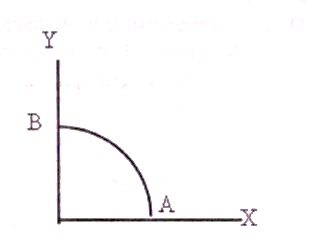
\includegraphics[width=0.23\textwidth]{Figs/image (4).png}
  \caption{}
  \label{fig:23}
\end{figure}

\begin{enumerate}
  \begin{multicols}{4}
  \item $-\dfrac{\pi}{2} - 1$
  \item $\dfrac{\pi}{2} + 1$
  \item $\dfrac{\pi}{2}$
  \item $1$
  \end{multicols}
\end{enumerate}
\hfill{\brak{\text{GATE ME 2009}}}


%24
\item The distance between the origin and the point nearest to it on the surface $z^2 = 1+xy$ is
\begin{enumerate}
  \begin{multicols}{4}
  \item $1$
  \item $\frac{\sqrt{3}}{2}$
  \item $\sqrt{3}$
  \item $2$
  \end{multicols}
\hfill{\brak{\text{GATE ME 2009}}}
\end{enumerate}

%25
\item The area enclosed between the curves $y^2 = 4x$ and $x^2 = 4y$ is
\begin{enumerate}
  \begin{multicols}{4}
  \item $\frac{16}{3}$
  \item $8$
  \item $\frac{32}{3}$
  \item $16$
  \end{multicols}
\hfill{\brak{\text{GATE ME 2009}}}
\end{enumerate}

%26
\item The standard deviation of a uniformly distributed random variable between 0 and 1 is
\begin{enumerate}
  \begin{multicols}{4}
  \item $\dfrac{1}{\sqrt{12}}$
  \item $\dfrac{1}{\sqrt{3}}$
  \item $\dfrac{5}{\sqrt{12}}$
  \item $\dfrac{7}{\sqrt{12}}$
  \end{multicols}
\hfill{\brak{\text{GATE ME 2009}}}
\end{enumerate}

%27
\item Consider steady, incompressible and irrotational flow through a reducer in a horizontal pipe where the diameter is reduced from 20 cm to 10 cm. The pressure in the 20 cm pipe just upstream of the reducer is 150 kPa. The fluid has a vapour pressure of 50 kPa and a specific weight of 5 kN/m$^3$. Neglecting frictional effects, the maximum discharge $\brak{\text{in} m^3/s}$ that can pass through the reducer without causing cavitation is
\begin{enumerate}
  \begin{multicols}{4}
  \item $0.05$
  \item $0.16$
  \item $0.27$
  \item $0.38$
  \end{multicols}
\hfill{\brak{\text{GATE ME 2009}}}
\end{enumerate}

%28
\item In a parallel flow heat exchanger operating under steady state, the heat capacity rates of the hot and cold fluid are equal. The hot fluid, flowing at 1 kg/s with $C_p = 4$ kJ/kgK, enters at $102^\degree$C while the cold fluid has an inlet temp of $15^\degree$C. The overall heat transfer coefficient is $1$ kW/m$^2$K and area is 5 m$^2$. Neglect ambient heat transfer. The exchanger is characterized by $2\varepsilon = 1 - \exp(-2 NTU)$. The exit temperature (in $^\degree$C) for the cold fluid is
\begin{enumerate}
  \begin{multicols}{4}
  \item $45$
  \item $55$
  \item $65$
  \item $75$
  \end{multicols}
\hfill{\brak{\text{GATE ME 2009}}}
\end{enumerate}

%29
\item In an air-standard Otto cycle, the compression ratio is 10. The condition at the beginning of the compression process is 100 kPa and $27^\degree$C. Heat added at constant volume is $1500$ kJ/kg, while $700$ kJ/kg of heat is rejected during the other constant volume process. Specific gas constant for air = $0.287$ kJ/kgK. The mean effective pressure $\brak{\text{in} \ kPa}$ is
\begin{enumerate}
  \begin{multicols}{4}
  \item $103$
  \item $310$
  \item $515$
  \item $1032$
  \end{multicols}
\hfill{\brak{\text{GATE ME 2009}}}
\end{enumerate}

%30
\item An irreversible heat engine extracts heat from a high temperature source at 100 kW and rejects heat at 50 kW. The entire work output is used to drive a reversible heat pump operating between 17$^\degree$C and 75$^\degree$C. The rate \brak{\text{in} \  kW} at which the heat pump delivers heat to its high temp sink is
\begin{enumerate}
  \begin{multicols}{4}
  \item $50$
  \item $250$
  \item $300$
  \item $360$
  \end{multicols}
\hfill{\brak{\text{GATE ME 2009}}}
\end{enumerate}

%31
\item You are asked to evaluate assorted fluid flows for their suitability in a given laboratory application.
The following three flow choices, expressed in terms of the two-dimensional velocity fields in the
xy-plane, are made available.\\
\begin{enumerate}
 \item[P.] $u =2y, v =-3x$
 \item[Q.] $u =3xy, v = 0$
 \item[R.] $u=-2x, v=2y$
\end{enumerate}


Which flow(s) should be recommended when the application requires the flow to be incompressible and
irrotational?

\begin{enumerate}
  \begin{multicols}{4}
  \item P and R
  \item Q
  \item Q and R
  \item R
  \end{multicols}
\hfill{\brak{\text{GATE ME 2009}}}
\end{enumerate}

%32
\item Water at 25$^\degree$C flows through a 1.0 km long G.I. pipe of 200 mm diameter at $0.07$ m$^3$/s. Darcy friction factor is 0.02 and water density is 1000 kg/m$^3$. The pumping power $\brak{\text{in} \ kW}$ required is
\begin{enumerate}
  \begin{multicols}{4}
  \item $1.8$
  \item $17.4$
  \item $20.5$
  \item $41.0$
  \end{multicols}
\hfill{\brak{\text{GATE ME 2009}}}
\end{enumerate}

%33
\item Steady-state heat conduction across the thickness in a plane composite wall (see figure) exposed to convection on both sides\\Given: $h_1 = 20$ W/m$^2$K; $h_2 = 50$ W/m$^2$K; $T_{\infty,1}=20^\degree$C; $T_{\infty,2}=-2^\degree$C; $k_1 = 20$ W/mK; $k_2 = 50$ W/mK; $L_1 = 0.30$ m, $L_2 = 0.15$ m. Assuming negligible contact resistance between the wall surfaces, the interface temperature,$T$ \brak{\text{in} ^\degree C}, of the two walls will be 
\begin{figure}[h]
  \centering
  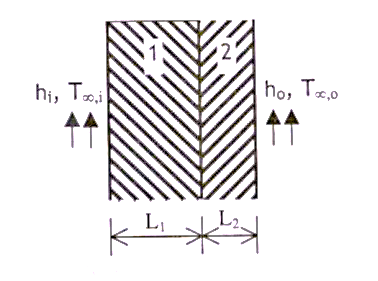
\includegraphics[width=0.23\textwidth]{Figs/image (5).png}
  \caption{}
  \label{fig:33}
\end{figure}


\begin{enumerate}
  \begin{multicols}{4}
  \item $-0.50$
  \item $2.75$
  \item $3.75$
  \item $4.50$
  \end{multicols}
\hfill{\brak{\text{GATE ME 2009}}}
\end{enumerate}



%34
\item The velocity profile of a fully developed laminar flow in a straight circular pipe, as shown in the figure, is given by the expression
\begin{align}
    u(r) = \frac{R^2}{4\mu} \frac{dp}{dx} \left(1 - \frac{r^2}{R^2}\right)
\end{align}


where is a constant. The average velocity of fluid in the pipe is
\begin{figure}[h]
  \centering
  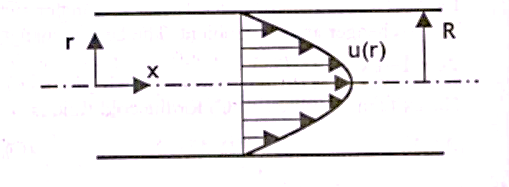
\includegraphics[width=0.5\textwidth]{Figs/image (6).png}
  \caption{}
  \label{fig:34}
\end{figure}


\begin{enumerate}
 \begin{multicols}{4}
  \item $\dfrac{R^2}{8\mu} \dfrac{dp}{dx}$
  \item $\dfrac{R^2}{4\mu} \dfrac{dp}{dx}$
  \item $\dfrac{R^2}{6\mu} \dfrac{dp}{dx}$
  \item $\dfrac{R^2}{2\mu} \dfrac{dp}{dx}$
  \end{multicols}
\hfill{\brak{\text{GATE ME 2009}}}
\end{enumerate}





%35
\item A solid shaft of diameter, d and length, L is fixed at both the ends. A torque, To is applied at a distance,
L/4 from the left end as shown in the figure given below.


\begin{figure}[h]
  \centering
  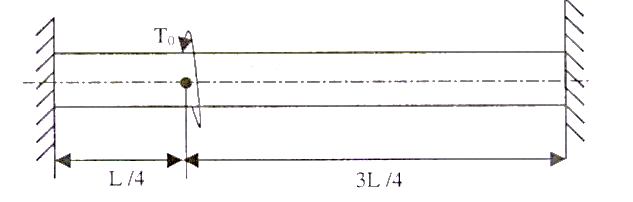
\includegraphics[width=0.5\textwidth]{Figs/image (7).png}
  \caption{}
  \label{fig:35}
\end{figure}

The maximum shear stress in the shaft is

\begin{enumerate}
  \begin{multicols}{4}
  \item $\frac{16T_0}{3\pi d^3}$
  \item $\frac{12T_0}{\pi d^3}$
  \item $\frac{8T_0}{\pi d^3}$
  \item $\frac{4T_0}{3\pi d^3}$
  \end{multicols}
\hfill{\brak{\text{GATE ME 2009}}}
\end{enumerate}




%36
\item An epicyclic gear train is shown schematically in the adjacent figure. The sun gear 2 on the input shaft is a 20 teeth external gear. The planet gear 3 is a 40 teeth external gear. The ring gear 5 is a 100 teeth internal gear. The ring gear 5 is fixed and gear 2 is rotating at 60 rpm ccw. The arm 4 attached to the output shaft will rotate at
\begin{figure}[h] 
  \centering
  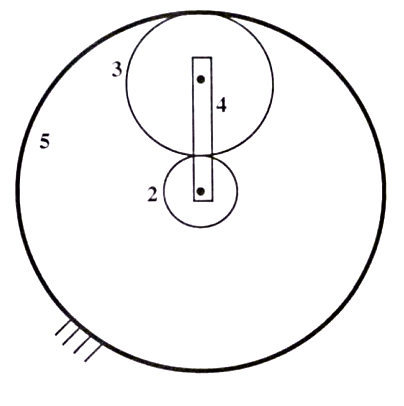
\includegraphics[width=0.23\textwidth]{Figs/image (8).png}
  \caption{}
  \label{fig:36}
\end{figure}

\begin{enumerate}
  \begin{multicols}{4}
  \item 10 rpm ccw
  \item 10 rpm cw
  \item 12 rpm cw
  \item 12 rpm ccw
  \end{multicols}
\hfill{\brak{\text{GATE ME 2009}}}
\end{enumerate}

%37
\item A forged steel link with uniform diameter of 30 mm at the centre is subjected to an axial force that varies from 40 kN in compression to 160 kN in tension. The tensile ($S_u$), yield ($S_y$) and corrected endurance ($S_e$) strengths of the steel are 600 MPa, 420 MPa, and 240 MPa respectively. The factor of safety against fatigue endurance as per Soderberg's criterion is
\begin{enumerate}
  \begin{multicols}{4}
  \item 1.26
  \item 1.37
  \item 1.45
  \item 2.00
  \end{multicols}
\hfill{\brak{\text{GATE ME 2009}}}
\end{enumerate}

%38
\item An automotive engine weighing 240 kg is supported on four springs with linear characteristics. Each of the front two springs have a stiffness of 16 MN/m while the stiffness of each rear spring is 32 MN/m. The engine speed $\brak{\text{in}\  rpm}$, at which resonance is likely to occur, is
\begin{enumerate}
  \begin{multicols}{4}
  \item 6040
  \item 3020
  \item 1424
  \item 955
  \end{multicols}
\hfill{\brak{\text{GATE ME 2009}}}
\end{enumerate}

%39
\item A vehicle suspension system consists of a spring and a damper. The stiffness of the spring is 3.6 kN/m and the damping constant is 400 Ns/m. If the mass is 50 kg, then the damping factor ($d$) and damped natural frequency ($f_n$), respectively, are
\begin{enumerate}
  \item 0.471 and 1.19 Hz
  \item 0.471 and 7.48 Hz
  \item 0.666 and 1.35 Hz
  \item 0.666 and 8.50 Hz
\hfill{\brak{\text{GATE ME 2009}}}
\end{enumerate}

%40
\item A frame of two arms of equal length $L$ is shown in the adjacent figure. The flexural rigidity of each arm of the frame is $EI$. The vertical deflection at the point of application of load $P$ is
\begin{figure}[h]
  \centering
  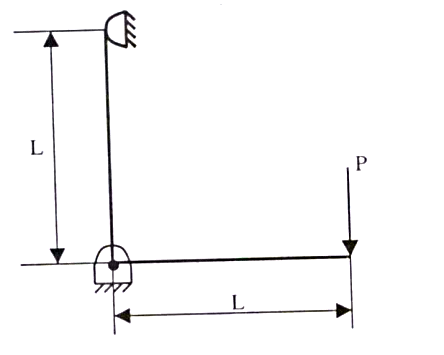
\includegraphics[width=0.5\textwidth]{Figs/image (9).png}
  \caption{}
  \label{fig:40}
\end{figure}

\begin{enumerate}
  \begin{multicols}{4}
  \item $\frac{PL^3}{3EI}$
  \item $\frac{2PL^3}{3EI}$
  \item $\frac{PL^3}{EI}$
  \item $\frac{4PL^3}{3EI}$
  \end{multicols}
\hfill{\brak{\text{GATE ME 2009}}}
\end{enumerate}





%41
\item A uniform rigid rod of mass $M$ and length $L$ is hinged at one end as shown in the adjacent figure. A force $P$ is applied at a distance $\dfrac{2L}{3}$ from the hinge so that the rod swings to the right. The reaction at the hinge is
\begin{figure}[h]
  \centering
  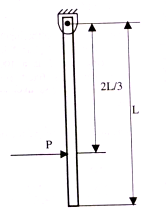
\includegraphics[width=0.23\textwidth]{Figs/image (10).png}
  \caption{}
  \label{fig:41}
\end{figure}
\begin{enumerate}
  \begin{multicols}{4}
  \item $-P$
  \item $0$
  \item $\dfrac{P}{3}$
  \item $\dfrac{2P}{3}$
  \end{multicols}
\hfill{\brak{\text{GATE ME 2009}}}
\end{enumerate}
 %42
\item Match the approaches given below to perform stated kinematics /dynamics analysis of machine.\\
\begin{table}[h]
    \centering
    \begin{center}
\begin{tabular}{ll}
    \textbf{Group I} & \textbf{Group II} \\
    P. Ferrite & 1. Hexagonal Close Packed (HCP) \\
    Q. Austenite & 2. Body Centered Cubic (BCC) \\
    R. Martensite & 3. Body Centered Tetragonal (BCT) \\
    & 4. Face Centered Cubic (FCC)
\end{tabular}
\end{center}
\end{table}\\

\begin{enumerate}
  \item P-1, Q-2, R-3, S-4
  \item P-3, Q-4, R-2, S-1
  \item P-2, Q-3, R-4, S-1
  \item P-4, Q-2, R-1, S-3
\hfill{\brak{\text{GATE ME 2009}}}
\end{enumerate}

%43
\item A company uses 2555 units of an item annually. Delivery lead time is 8 days. The reorder point (in number of units) to achieve optimum inventory is
\begin{enumerate}
  \begin{multicols}{4}
  \item 7
  \item 8
  \item 56
  \item 60
  \end{multicols}
\hfill{\brak{\text{GATE ME 2009}}}
\end{enumerate}

%44
\item Consider the following Linear Programming Problem (LPP):
\begin{align*}
  \text{Maximize} \ z = 3x_1 + 2x_2 \\ \text{subject  to}\  x_1 \leq 4,\\\ x_2 \leq 6,\\\ 3x_1 + 2x_2 \leq 18,\\\ x_1, x_2 \geq 0.
\end{align*}
\\     The nature of this LPP is
\begin{enumerate}
  \item The LPP has a unique optimal solution.
  \item The LPP is infeasible.
  \item The LPP is unbounded.
  \item The LPP has multiple optimal solutions.
\hfill{\brak{\text{GATE ME 2009}}}
\end{enumerate}
\newpage
%45
\item Six jobs arrived in a sequence as given below:\\
\begin{table}[h]
    \centering
    \begin{tabular}{|c|c|c|}
     \hline
     \textbf{Mineral} & \textbf{Modal abundance \brak{\%}} & \textbf{Partition coefficient}\\
     \hline
     Clinopyroxene & $45$ & $0.506$ \\
      \hline
      Orthopyroxene & $40$ & $0.42$ \\
      \hline
      Olivine & $10$ & $0.045$ \\
      \hline
      Plagioclase & $05$ & $0.019$ \\
      \hline
\end{tabular}
\end{table}

Average flow time (in days) for the above jobs using Shortest Processing Time rule is
\begin{enumerate}
  \begin{multicols}{4}
  \item 20.83
  \item 23.16
  \item 125.00
  \item 139.00
  \end{multicols}
\hfill{\brak{\text{GATE ME 2009}}}
\end{enumerate}

%46
\item Minimum shear strain in orthogonal turning with a cutting tool of zero rake angle is
\begin{enumerate}
  \begin{multicols}{4}
  \item 0.0
  \item 0.5
  \item 1.0
  \item 2.0
  \end{multicols}
\hfill{\brak{\text{GATE ME 2009}}}
\end{enumerate}


%47
\item Electrochemical machining is performed to remove material from an iron surface of 20 mm $\times$ 20 mm under the following conditions: 
\begin{center}
    Inter electrode gap = 0.2 mm\\
    Supply voltage = 12 V\\
    Specific resistance of electrolyte = 2$\Omega$cm\\
    Atomic weight of iron = 55.85\\
    Valency of Iron = 2\\
    Faraday's constant = 96540 C\\
\end{center}
The material removal rate $\brak{\text{in} g/s}$ is
\begin{enumerate}
  \begin{multicols}{4}
  \item 0.3471
  \item 3.471
  \item 34.71
  \item 347.1
  \end{multicols}
\hfill{\brak{\text{GATE ME 2009}}}
\end{enumerate}

%48
\item Match the following:\\
\begin{table}[h]
    \centering
    \begin{table}[htbp]
  \centering
  \caption{Table-3}
  \label{table3}
  \begin{tabular}{cc}
  \textbf{Processing Technique} & \textbf{Producct} \\ \\
    P. Calendering & 1. Pipes \\
    Q. Extrusion & 2. Disposable cups \\
    R. Injection moulding & 3. Sheets \\
    S. Thermoforming & 4. Nylon gears \\
  \end{tabular}
\end{table}
    
\end{table}
\begin{enumerate}
  \item P-2, Q-3, R-4, S-1
  \item P-3, Q-4, R-2, S-1
  \item P-3, Q-4, R-1, S-2
  \item P-4, Q-3, R-2, S-1
\hfill{\brak{\text{GATE ME 2009}}}
\end{enumerate}

%49
\item What are the upper and lower limits of the shaft represented by 60 fg?\\ Use the following data:
\\ Diameter 60 lies in the diameter step of 50-80 mm. \\
Fundamental tolerance unit $i$ in $\mu$m $= 0.45 D^{1/3} + 0.001 D$, where $D$ is the representative size in mm; \\
Tolerance value for IT8 $= 25i$. Fundamental deviation for 'f' shaft $= -5.5 D^{0.41}$
\begin{enumerate}
  \item Lower limit = 59.924 mm, Upper Limit = 59.970 mm
  \item Lower limit = 59.954 mm, Upper Limit = 60.000 mm
  \item Lower limit = 59.970 mm, Upper Limit = 60.016 mm
  \item Lower limit = 60.000 mm, Upper Limit = 60.046 mm
\hfill{\brak{\text{GATE ME 2009}}}
\end{enumerate}

%50
\item Match the items in Column I and Column II:\\
\begin{table}[h]
    \centering
    \begin{center}
\begin{tabular}{|c|c|c|}
    \hline
    Task & Task time (Seconds) & Immediate predecessor(s) \\
    \hline
    P & 20 & - \\ \hline
    Q & 25 & P \\  \hline
    R & 10 & Q \\ \hline
    S & 15 & Q \\ \hline 
    T & 25 & R, S \\    \hline
\end{tabular}
\end{center}
   
\end{table}
\begin{enumerate}
  \item P-1, Q-3, R-2, S-4
  \item P-3, Q-4, R-2, S-1
  \item P-1, Q-4, R-2, S-3
  \item P-4, Q-1, R-2, S-3
  \hfill{\brak{\text{GATE ME 2009}}}
\end{enumerate}

\textbf{Common Data Questions}

\textbf{Common Data for Questions 51 and 52:}

The inlet and the outlet conditions of steam for an adiabatic steam turbine are as indicated in the\\
The notations are as usually followed.
\begin{figure}[h]
  \centering
  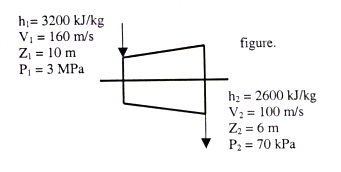
\includegraphics[width=0.5\textwidth]{Figs/image (11).png}
  \caption{}
  \label{fig:50}
\end{figure}

%51
\item If mass flow rate of steam through the turbine is 20 kg/s, the power output of the turbine $\brak{\text{in} MW}$ is
\begin{enumerate}
  \begin{multicols}{4}
  \item 12.157
  \item 12.941
  \item 168.001
  \item 168.785
  \end{multicols}
\hfill{\brak{\text{GATE ME 2009}}}
\end{enumerate}

%52
\item Assume the above turbine to be part of a simple Rankine cycle. The density of water at the inlet to the pump is 1000 kg/m$^3$. Ignoring kinetic and potential energy effects, the specific work $\brak{\text{in} \  kJ/kg}$ supplied to the pump is
\begin{enumerate}
  \begin{multicols}{4}
  \item 0.293
  \item 0.351
  \item 2.930
  \item 3.510
  \end{multicols}
\hfill{\brak{\text{GATE ME 2009}}}
\end{enumerate}

\textbf{Common Data for Questions 53 and 54:}\\
Radiative heat transfer is intended between the inner surfaces of two very large isothermal parallel metal plates. The upper plate (plate 1) is a black surface and is the warmer, maintained at $727^{\degree}$C. The lower plate (plate 2) is diffuse and gray with emissivity 0.7 and kept at $227^{\degree}$C. Assume sufficiently large surfaces and steady-state; Stefan-Boltzmann constant is $5.67 \times 10^{-8}$ W/m$^2$K$^4$.
%53
\item The irradiation $\brak{\text{in}\  kW/m^2}$ for the upper plate (plate 1) is
\begin{enumerate}
  \begin{multicols}{4}
  \item 2.5
  \item 3.6
  \item 17.0
  \item 19.5
  \end{multicols}
\hfill{\brak{\text{GATE ME 2009}}}
\end{enumerate}
%54
\item If plate 1 is also diffuse and gray with emissivity 0.8, the net radiation heat exchange \brak{\text{in} \ kW/m^2} between plates 1 and 2 is
\begin{enumerate}
  \begin{multicols}{4}
  \item 17.0
  \item 19.5
  \item 23.0
  \item 31.7
  \end{multicols}
\hfill{\brak{\text{GATE ME 2009}}}
\end{enumerate}
\textbf{Common Data for Questions 55 and 56 :}\\
Consider the following PERT network:
\begin{figure}[h]
  \centering
  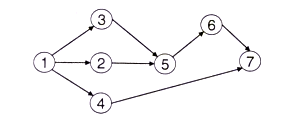
\includegraphics[width=0.5\textwidth]{Figs/image (12).png}
  \caption{}
  \label{fig:54}
\end{figure}
The optimistic time, most likely time and pessimistic time of all the activities are given in the table below:\\
\begin{table}[h]
    \centering
    \begin{center}
\begin{tabular}{|c|c|c|}
    \hline
    Task & Task time (Seconds) & Immediate predecessor(s) \\
    \hline
    P & 20 & - \\ \hline
    Q & 25 & P \\  \hline
    R & 10 & Q \\ \hline
    S & 15 & Q \\ \hline 
    T & 25 & R, S \\    \hline
\end{tabular}
\end{center}
   
\end{table}
\newpage


%55
\item The critical path duration of the network (in days) is
\begin{enumerate}
  \begin{multicols}{4}
  \item 11
  \item 14
  \item 17
  \item 18
  \end{multicols}
\hfill{\brak{\text{GATE ME 2009}}}
\end{enumerate}
%56
\item The standard deviation of the critical path is
\begin{enumerate}
  \begin{multicols}{4}
  \item 0.33
  \item 0.55
  \item 0.77
  \item 1.66
  \end{multicols}
\hfill{\brak{\text{GATE ME 2009}}}
\end{enumerate}

\textbf{Linked Answer Questions}\\
\textbf{Statement for Linked Answer Questions 57 and 58:}\\
In a machining experiment, tool life was found to vary with the cutting speed in the following manner:
\begin{table}[h]
    \centering
    \begin{table}[htbp]
  \centering
  \caption{Table-6}
  \label{tab:tables/table6.tex}
  \begin{tabular}{cc}
  \textbf{Reagent} & \textbf{Function} \\ \\
    P.Ammonia  & 1. Prevent storage hardening \\
    Q. Hydroxylamine & 2. Delay plugging mechanism \\
    R. Formic acid & 3. Stabilizer \\
    S. Ethephone & 4. Coagulating agent \\
  \end{tabular}
\end{table}
   
\end{table}

%57
\item The exponent $(n)$ and constant $(k)$ of Taylor's tool life equation are
\begin{enumerate}
  \item $n=0.5$ and $k=540$
  \item $n=-1$ and $k=0.74$
  \item $n=1$ and $k=4860$
  \item $n=-0.5$ and $k=1.155$
\hfill{\brak{\text{GATE ME 2009}}}
\end{enumerate}

%58
\item What is the percentage increase in tool life when cutting speed is halved?
\begin{enumerate}
  \begin{multicols}{4}
  \item 50\%
  \item 200\%
  \item 300\%
  \item 400\%
  \end{multicols}
\hfill{\brak{\text{GATE ME 2009}}}
\end{enumerate}

\textbf{Statement for Linked Answer Questions 59 and 60:}\\
A 20° full depth involute spur pinion of 4 mm module and 21 teeth is to transmit 15 kW at 960 rpm. Its face width is 25 mm.
\item The tangential force transmitted $(in\  N)$ is
\begin{enumerate}
  \begin{multicols}{4}
  \item 3552
  \item 2611
  \item 1776
  \item 1305
  \end{multicols}
\end{enumerate}

%60
\item Given the tooth geometry factor is $0.32$ and combined effect of dynamic load and allied factors intensifying stress is $1.5$, the minimum allowable stress $(in\  MPa)$ for the gear material is
\begin{enumerate}
  \begin{multicols}{4}
  \item 242.0
  \item 166.5
  \item 121.0
  \item 74.0
  \end{multicols}
\hfill{\brak{\text{GATE ME 2009}}}
\end{enumerate}



\end{enumerate}

\end{document}
